%_____________________________________________________________________________________
%
%       Filename:  chapter4.tex
%
%    Description:  Thesis Template HS Offenburg
%
%
%         Author:  Okba ZOUEGHI, okba.zoueghi@gmail.com
%     Supervisor:  Andreas Walz, Chadlia Jerad
%   Organization:  HS Offenburg, Offenburg, Germany
%
%_____________________________________________________________________________________

\chapter{Design}

% During this chapter, we start by specifying the functional and non-functional requirements
% then pass to

In this chapter, we provide and discuss the candidate solutions for integrating the DTLS
protocol within SafetyNETp RTFN communication model. Our security layer DTLS-based design is
discussed in two parts. In the first part, we see the global design in which we discuss
the handshake timing, DTLS and SafetyNETp role mapping as well as the secure channel creation.
The second part is the detailed design, in this section, we go deeper into the solutions to
see the security layer positioning, how the outgoing and incoming message are treated,
the frame layout as well as several other details.

\section{Global Design}

As we mentioned before it is easy to provide a secure channel for an application layer
protocol by inserting DTLS or TLS (based on the underlying transport layer) between the application
layer and the transport layer. For instance, \ac{HTTPS} is a secure version
of \ac{HTTP}, this security is provided by inserting TLS between TCP and \ac{HTTP}. This is made easy due to the
fact that \ac{HTTP} and TLS follow both the Client/Server communication model.

Unlike \ac{HTTP} and similar protocols, providing a DTLS-based security layer for SafetyNETp is not as simple as it seems.
In fact, SafetyNETp is based on Publish/Subscribe communication model, on the other hand, DTLS is designed for
Client/Server based applications. Hence, we need a solution which allows mapping and adapting
DTLS to SafetyNETp. Furthermore, an important question could be asked: in which step of SafetyNETp
communication the handshake should be established?

In this section, we see when the DTLS handshake is established, how to manage
mapping the roles for the different communication model and we present how a secure channel
is provided.

\subsection{When To Establish The Handshake?}


As shown in \autoref{when_to_establish_the_handshake}
there are three possible alternatives. Establish the handshake before sending a \textit{subscribe request}, after sending
a \textit{subscribe request} but before receiving an acknowledgment, and the last alternative after receiving an
acknowledgment. These cases correspond to the device which takes the subscriber role. Regarding
the publisher, there are two alternatives, whether after or before sending a \textit{subscribe acknowledgment}.

\begin{figure}[!htbp]
\centering
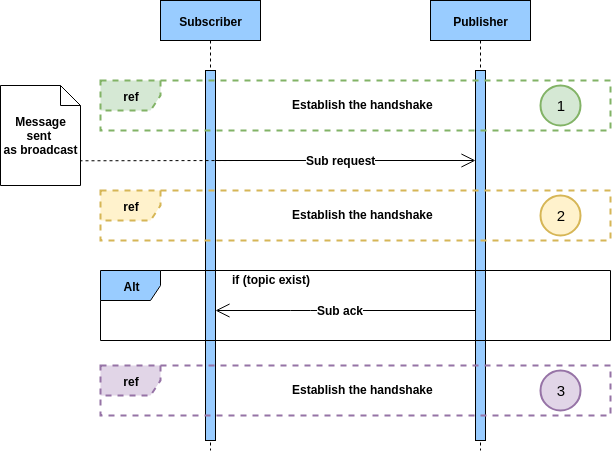
\includegraphics[width=12cm,height=9cm]{figures/design/when_to_establish_the_handshake.png}
\caption{Possible cases of handshake establishement}\label{when_to_establish_the_handshake}
\end{figure}

% As we mentioned before publishers and subscribers don't know each other in advance. Therefore
% the subscriber could not establish the handshake in the first and the second case because the publisher
% which is the second handshake end-point is unknown at this level. For the first two cases, the solution is to establish
% the handshake with all the devices. For that, the subscriber needs to know the possible ranges of IP addresses
% that can be used in the network. the advantage of this solution is that the first subscription
% process will be performed through the secure channel created after the handshake was established.
% However, this solution is not efficient in term of memory and bandwidth usage, in term of startup time
% and in term of flexibility.  For each handshake, memory resources need to be allocated which is memory
% waste because not all the channels will be used by the subscriber. To perform the handshake, if we assume
% for example that the subscriber has a client role, it sends Client Hello message to all the IP addresses
% existing in the used IP ranges. Therefore messages will be sent also to unused IP addresses which is
% bandwidth waste. The startup time will increase if the number of devices is important. Regarding the flexibility,
% if a new IP addresses range is used in the network, the devices need to be reconfigured.
%
%
% Regarding the third case, after that the subscriber receives a \textit{subscribe acknowledgment} from the publisher,
% at this level, the subscriber knows the second handshake end-point and the handshake could be established.
% The disadvantage of the previous solution is not present here. Only necessary channels will be created
% which optimizes the memory and the bandwidth usage and reduces the startup time. Furthermore,
% no information needed about the IP addresses ranges which allow more flexibility. Unfortunately,
% the first subscription process will not be authenticated in addition the publisher starts
% sending \textit{cyclic data} to the subscriber after sending the \textit{subscribe acknowledgment} which presents an issue.
% In fact the \textit{cyclic data} will be sent while the handshake is being established, however, the
% identity of the second end-point is not verified. Hence \textit{cyclic data} will be sent to untrusted devices.
%
% In the third case, the subscriber and the publisher know each other addresses which solves
% the problems present in the first and the second case. Comparing these alternatives, the third is better in term of
% memory, bandwidth, flexibility and startup time. Therefore we choose to establish the handshake after the first subscription process.
% We see in the next sections how we solve the authentication issue for the first subscription
% as well as sending \textit{cyclic data} to untrusted devices.

As we mentioned before publishers and subscribers don't know each other in advance. Therefore
the subscriber could not establish the handshake in the first and the second cases because the publisher
which is the second handshake end-point is unknown at this time. For the first two cases, the solution is to establish
the handshake with all the devices. The handshakes establishment is triggered by the devices' startup, therefore,
it is not possible to add a new device to the network at runtime. Assuming that we have a network of RTFN devices, at startup time,
all the devices will establish the handshake with each other and they start exchanging data. If we add a new device after this phase,
no handshake will be established with it as the handshakes phase has already finished, hence, the new device will not be able
to communicate securely. To be able to add a new device to the network, the devices should be restarted.
Furthermore, this solution is not efficient in term of memory usage and startup time.
For each handshake, memory resources need to be allocated which is memory
waste because not all the channels will be used by the subscriber.
Besides, the startup time will increase if the number of devices is important.
This method introduces another inconvenient, a session between a publisher and a subscriber should remain always open
even if no communication is needed. In fact, once the session is closed, they could not establish a new session
as it is triggered by the startup. Letting unnecessary sessions open leads to memory waste.


Regarding the third case, after that the subscriber receives a \textit{subscribe acknowledgment} from the publisher,
at this level, the subscriber knows the second handshake end-point and the handshake could be established.
The disadvantages of the previous solution are not present here. Only necessary channels will be created
which optimizes the memory usage and reduces the startup time. In addition unlike the previous cases,
unnecessary sessions could be closed as the handshake is triggered by the subscription process (more details about sessions closing are
given in the next sections). Unfortunately, our security layer
needs in this case to inspect the application layer header in order to take the decision.
Furthermore, the publisher starts
sending \textit{cyclic data} to the subscriber after sending the \textit{subscribe acknowledgment} which presents an issue.
In fact the \textit{cyclic data} will be sent while the handshake is being established, however, the
identity of the second end-point is not verified. Hence \textit{cyclic data} could be sent to untrusted devices.

The \autoref{alternatives_comparison} shows the main differences between the cited alternatives.

\begin{table}[H]
  \centering
    \begin{tabular}{|l|l|l|}
      \hline
      & First and second cases & Third case \\
      \hline
      Memory usage & more & less \\
      \hline
      Startup time & more & less \\
      \hline
      Message inspection & no & yes \\
      \hline
      Flexibility & no & yes \\
      \hline
      Close unnecessary sessions & no & yes \\
      \hline
      Cylic data sent while & &\\
      establishing the handshake & no & yes \\
      \hline
  \end{tabular}
  \caption{Alternatives comparison}\label{alternatives_comparison}
\end{table}


In the third case, the subscriber and the publisher know each other addresses which solves the problems present in the first and the second cases. Comparing these alternatives, the third is better in term of
flexibility, memory usage, and startup time. Therefore we choose to establish the handshake after the first subscription process.
We see in the next sections how to deal with the \textit{cyclic data} sent while the handshake is being established.


\subsection{SafetyNETp and DTLS Role Mapping}

After choosing when to establish the handshake, an important question could be asked.
How to map DTLS roles (client/server) with SafetyNETp roles (publisher/subscriber)?
The intuitive solution is that the subscriber takes the role of the client and the publisher
takes the role of the server. After sending the \textit{subscribe acknowledgment}, the publisher
activates its servers and waits for a Client Hello message. After receiving the subscribe
acknowledgment the subscriber takes the client role and sends a Client Hello to the publisher
which has already activated its server and which is ready to establish the handshake. Once the handshake
has finished successfully, the publisher can send \textit{cyclic data} securely through the created secure channel.


Unfortunately, if we consider that two SafetyNETp devices could have a mutual subscription,
an issue is presented. As shown in \autoref{simultaneous_mutual_subsribtion}, the devices A and B subscribe mutually to each other in parallel
at the same time. As discussed in the previous section the event which triggers the
handshake establishment is the subscription process. With the method presented above, having simultaneous
subscription will lead to create two channels between A and B. We will end up having a channel for each relation of
(publisher,subscriber). In the case shown in \autoref{simultaneous_mutual_subsribtion} we have two relations, the relation (A,B), in which A
is the publisher and B is the subscriber and the (B,A) relation which is the opposite. Therefore two
separate channels will be created between A and B whereas one single channel is sufficient.

Creating more than one channel for the same couple leads to more memory usage that's why
we need a mechanism to avoid duplicated channels. After that both of A and B had sent
the \textit{subscribe acknowledgment}, they know each other's IP addresses. Based on the IP addresses,
each device can choose a distinct DTLS role. The device which has the greater IP address
takes the server role, the other device takes the client role.
Therefore, we choose to use IP addresses as a criterion to map DTLS and SafetyNETp roles. Other alternatives
than the IP addresses could be used like MAC addresses for example. What is important is to make the choice and break the conflict
to avoid duplicated channels which could be achieved using this method.

\begin{figure}[H]
\centering
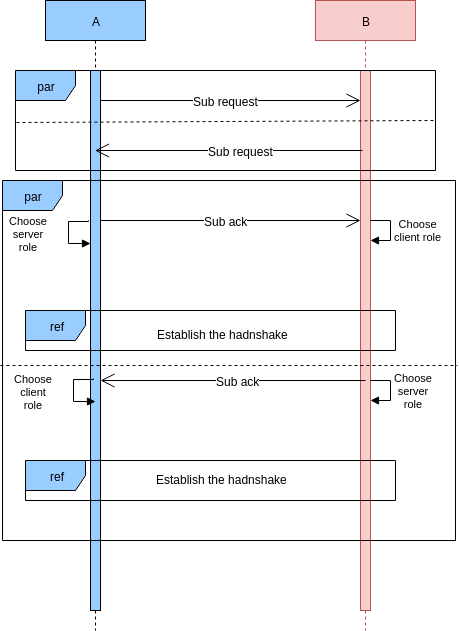
\includegraphics[width=9cm,height=9cm]{figures/design/mutual_subsribtion.png}
\caption{Simultaneous mutual subscription}\label{simultaneous_mutual_subsribtion}
\end{figure}

\subsection{Secure Communication}

As a first step, we discussed when to establish the handshake, as a second step
we defined a mechanism to map the client/server role with the publisher/subscriber role.
As mentioned before, if the handshake is established after the subscription process,
the publisher starts sending \textit{cyclic data} while the handshake is being established.
This can lead to send \textit{cyclic data} to unauthorized devices as the data is sent before finishing the handshake.
In this section, as a next step, we take into consideration this issue and then we see a nominal case of a secure communication between two devices

\textit{Cyclic data} messages are very important that's why they should not be sent or received from
an untrusted device. While the handshake is being established, for the publisher,
the identity of the subscriber is not verified yet. As mentioned in the non-functional
requirements, our security layer should not introduce any changes to SafetyNETp state machine, therefore, two decisions could be taken,
whether to drop or to store the \textit{cyclic data} until finishing the handshake. If the \textit{cyclic data}
is stored, once the handshake is finished and the identity is verified, nothing is lost and
the \textit{cyclic data} could be sent securely through the secure channel. However, storing the cyclic
data can eventually cause a DoS attack. In fact, an attacker could send a huge number
of \textit{subscribe request} to a publisher with spoofed IP addresses. The publisher will send
a \textit{subscribe acknowledgment} for each received request and then start storing the \textit{cyclic data}
until verifying the identities. Eventually, the identities will not be verified but the publisher
memory will become saturated and the publisher will be out of service. This is the first
reason for which the \textit{cyclic data} should not be stored, furthermore, the \textit{cyclic data} represent
information about a certain topic and based on its content subscribers take actions.
Having old information about a topic can cause serious problems, that's why we choose to drop
\textit{cyclic data} while establishing the handshake.

\begin{figure}[!htbp]
\centering
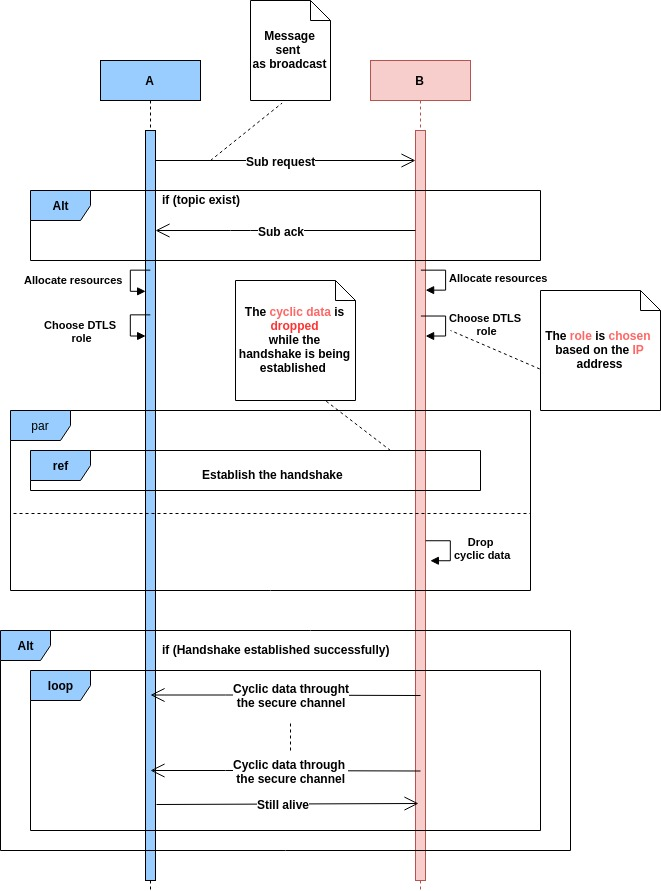
\includegraphics[width=11cm,height=15cm]{figures/design/nominal_case_for_secure_communication.jpg}
\caption{Nominal case of a secure communication}\label{nominal_case_for_secure_communication}
\end{figure}



The \autoref{nominal_case_for_secure_communication} illustrates a nominal case of a secure communication between two SafetyNETp devices.
Once the subscription process is done, both of the devices allocate the necessary memory needed for the
secure channel and then they choose DTLS roles based on their IP addresses. The handshake then starts, and the \textit{cyclic data}
is dropped. Once the handshake is finished successfully, sending the \textit{cyclic data} is resumed to be sent
through the secure channel.

\section{Detailed Design}

\subsection{Security Layer Positioning}

In this section, we see the positioning of the security layer and SafetyNETp in the TCP/IP model
and we discuss according to the messages' types whether a message should be sent through the security layer
or not.

As illustrated in \autoref{the_security_layer_and_safetynetp_in_tcp_ip_model}, the security layer is between UDP (transport layer) and SafetyNETp (application layer).
Sending a SafetyNETp application message can follow two paths, whether to be packed directly into a UDP datagram
or packed into our security layer frame and then into UDP. One can ask why would we enable SafetyNETp to skip the security layer
and use directly UDP. As we saw before in order to switch to a secure communication, the DTLS handshake need to be established.
The trigger of the handshake establishment is the first subscription process that's why the first subscription messages are sent
unprotected because at this level no secure channel exists.

\begin{figure}[H]
\centering
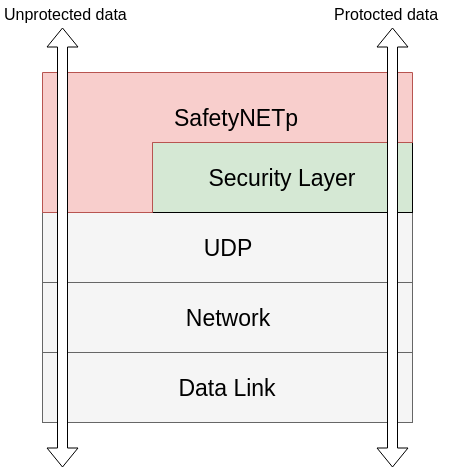
\includegraphics[height=7cm]{figures/design/the_security_layer_and_safetynetp_in_tcp_ip_model.png}
\caption{The security layer and SafetyNETp in TCP/IP model}\label{the_security_layer_and_safetynetp_in_tcp_ip_model}
\end{figure}

Once The handshake is established, a secure channel is provided and data could be exchanged securely but what are the
messages that should be sent through the secure channel? Do all of them should be sent securely?
Regarding \textit{subscribe requests} and \textit{acknowledgments} they obviously need to be sent securely, otherwise, a fake
\textit{subscribe request} could be sent and unnecessary data will be exchanged which leads to more CPU processing in both sides
(publisher and subscriber) and more bandwidth usage.
Actually, an attacker could use the fact that the subscription messages are unprotected. Being unprotected means that no integrity checks are
performed, therefore, if an attacker modifies the content of a message, the modification will not be detected.
A possible attack is shown in \autoref{man_in_the_middle_attack_exploiting_unprotected_subsribtion}, in this example, the attacker could modify the content of the packets with
a man in the middle attack. When the subscriber sends a \textit{subscribe request} for a topic X, the attacker
intercepts the messages and modifies it by changing the topic to Y. When the publisher receives the message it
sends back an acknowledgment and starts sending \textit{cyclic data} for topic Y which is not needed by the subscriber.
Moreover, an attacker could entirely forge and send fake \textit{subscribe requests} and, therefore, the bandwidth could be saturated.
The \textit{subscribe requests} are sent as broadcast to all the devices present on the network as the topic owner is
unknown in advance. Each secure channel corresponds to a couple of a publisher and a subscriber and there is no
secure channel shared between all the devices. Therefore, \textit{subscribe request} messages could not be sent securely as broadcast.
In order to avoid the previous problem, alongside sending the \textit{subscribe requests} as broadcast, the subscriber also
sends the same \textit{subscribe requests} as unicast and secured to the publishers with which it has an available secure channel.
When a publisher receives a \textit{subscribe request} as broadcast and unprotected from a subscriber, if it has an available
secure channel, the publisher ignore the subscribe request. If the publisher has no channel, it goes through the handshake establishment.
Hence, the publisher could avoid sending \textit{cyclic data} when receiving a tampered or a forged subscribe request.

\begin{figure}[H]
\centering
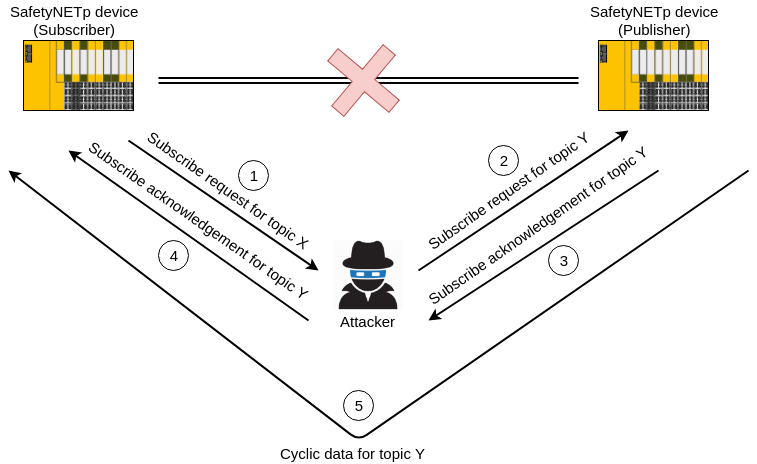
\includegraphics[height=7.5cm]{figures/design/man_in_the_middle_attack.png}
\caption{Man in the middle attack exploiting unprotected subscription}\label{man_in_the_middle_attack_exploiting_unprotected_subsribtion}
\end{figure}

As the rest of the messages are sent as unicast, they could be secured easily unlike the \textit{subscribe request} message.
The \textit{unsubscribe} and \textit{unpublished} messages could cause
issues if they are unprotected. In fact, an attacker could send a fake \textit{unsubscribe request} to a publisher
which will stop sending \textit{cyclic data} upon receiving the message. The last message type is the \textit{still alive} message,
as we discussed before it is used by the subscriber to inform the publisher that it is still alive. Therefore,
if it is sent unprotected, when a subscriber reboots for example, an attacker can send \textit{still alive} messages
to the list of publishers communicating with the subscriber. Hence they will not detect that the subscriber is down.
To conclude after analyzing the situation for each message type, once the handshake is established all
the messages should be sent through the secure channel.

\subsection{Flowcharts for Outgoing Messages}

In any SafetyNETp device using our security layer, whether the device is a publisher or a subscriber,
each outgoing message should follow the flowchart in \autoref{outgoing_messages_flowtchart}.

Let's take the example of two SafetyNETp devices, a subscriber
and a publisher respectively A and B. Initially, before starting the communication, no secure channel is available.
The communication starts when A sends a \textit{subscribe request} to B. The \textit{subscribe requests} are sent
unprotected as broadcast following the Path 4 and as no secure channel exists, no \textit{subscribe request} will be sent protected at this level.

Upon receiving the \textit{subscribe request}, like A, B will verify first if there is a secure channel for A.
Obviously, no secure channel exists, therefore, the \textit{subscribe acknowledgment} is sent unprotected and Path 1 is followed.
After sending the \textit{subscribe acknowledgment}, B will allocate the necessary resources and launch the handshake.
If the handshake is launched as a server, B will just wait for Client Hello messages coming from A, if it is
launched as a client, B will start sending Client Hello messages to A. Following the \textit{subscribe acknowledgment},
B will start sending \textit{cyclic data}. In this level, the handshake is being established, which means the identity of A
is not verified yet. The \textit{cyclic data} should be dropped, hence, Path 2 is followed. While establishing the handshake,
each \textit{cyclic data} message will follow Path 2 until it is finished. Once the first handshake is
established (we will have more than one handshake, more
details are given this in the next sections), every message is switched to be sent through the secure
channel. All the messages except \textit{subscribe requests} are sent following path 5. After that the handshake is established,
following the path 4, the \textit{subscribe requests} are sent unprotected as broadcast and secured as unicast through all the available channels.
In this case, If A performs another subscription after that the handshake is established, B will receive two subscribe requests
for the same topic, one as unicast through the security layer, and the other original unprotected broadcast subscribe request.
Obviously B, ignore the one sent as broadcast and process only the secured request. As we mentioned before,
sending \textit{subscribe requests} secured as unicast, enables the publisher to avoid responding for tampered and forged subscribe requests.

The path 3 shows how messages other than \textit{subscribe requests} and \textit{cyclic data} are sent before and while establishing the handshake.

\begin{figure}[p]
\centering
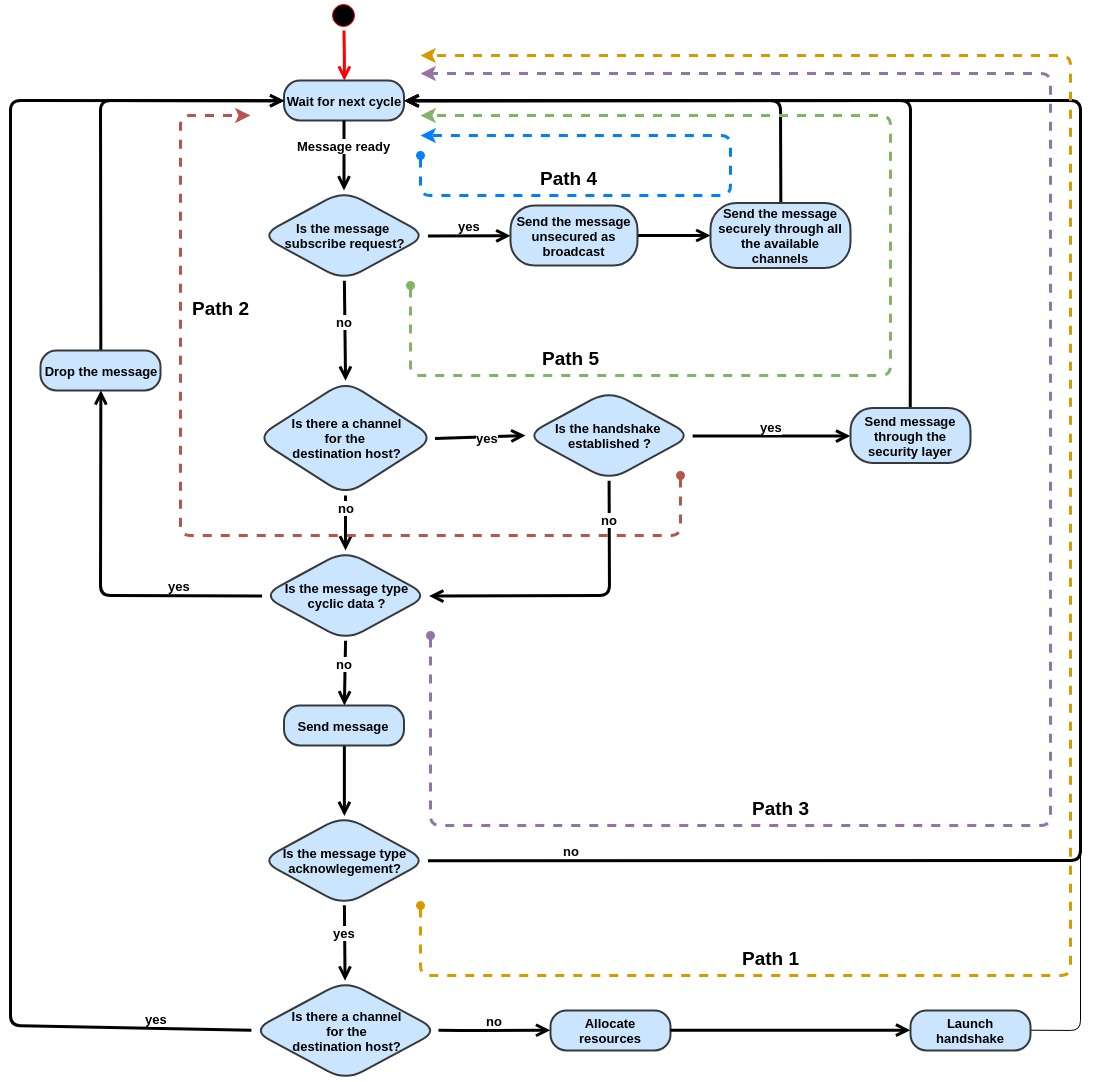
\includegraphics[height=16cm]{figures/design/outgoing_messages_flowtchart.jpg}
\caption{Flowchart for outgoing messages}\label{outgoing_messages_flowtchart}
\end{figure}

\newpage
\subsection{Flowchart for Incoming Messages}

Following the flowchart in \autoref{outgoing_messages_flowtchart} we ensure a secure encrypted and authenticated
communication in which messages are sent only to authorized devices, However, this flowchart does not include
the flow for received messages. The flowchart in \autoref{incoming_messages_flowtchart} illustrates how each incoming message is treated.

When \textit{cyclic data} is received and no secure channel is available, the message is dropped as shown in Path 1.
If we assume that we have a subscriber and a publisher respectively A and B, after sending a \textit{subscribe request}, A
will receive the first \textit{subscribe acknowledgment}. Upon receiving it, as no channel exists, A will allocate
the necessary resources and launch the handshake (Path 2). Meanwhile, if a \textit{cyclic data} message is received it
will be dropped as the identity of B is not verified yet (Path 1).

Once the first handshake is established, A and B will switch to
communicate via the secure channel. When a message is received the identity of the sender as well as
the message integrity will be verified. If the message is verified correctly, it will be decrypted and passed to SafetyNETp
application layer to get processed (Path 3). If the message is not verified it will be dropped (Path 4).

When an attacker impersonates the identity of B for example and sends a \textit{cyclic data} message to A,
if no secure channel is available, the message will be dropped (Path 1). After the handshake is established, if the attacker
finds a way to modify messages, the integrity checks will fail and the message will be dropped (Path 4).

\begin{figure}[p]
\centering
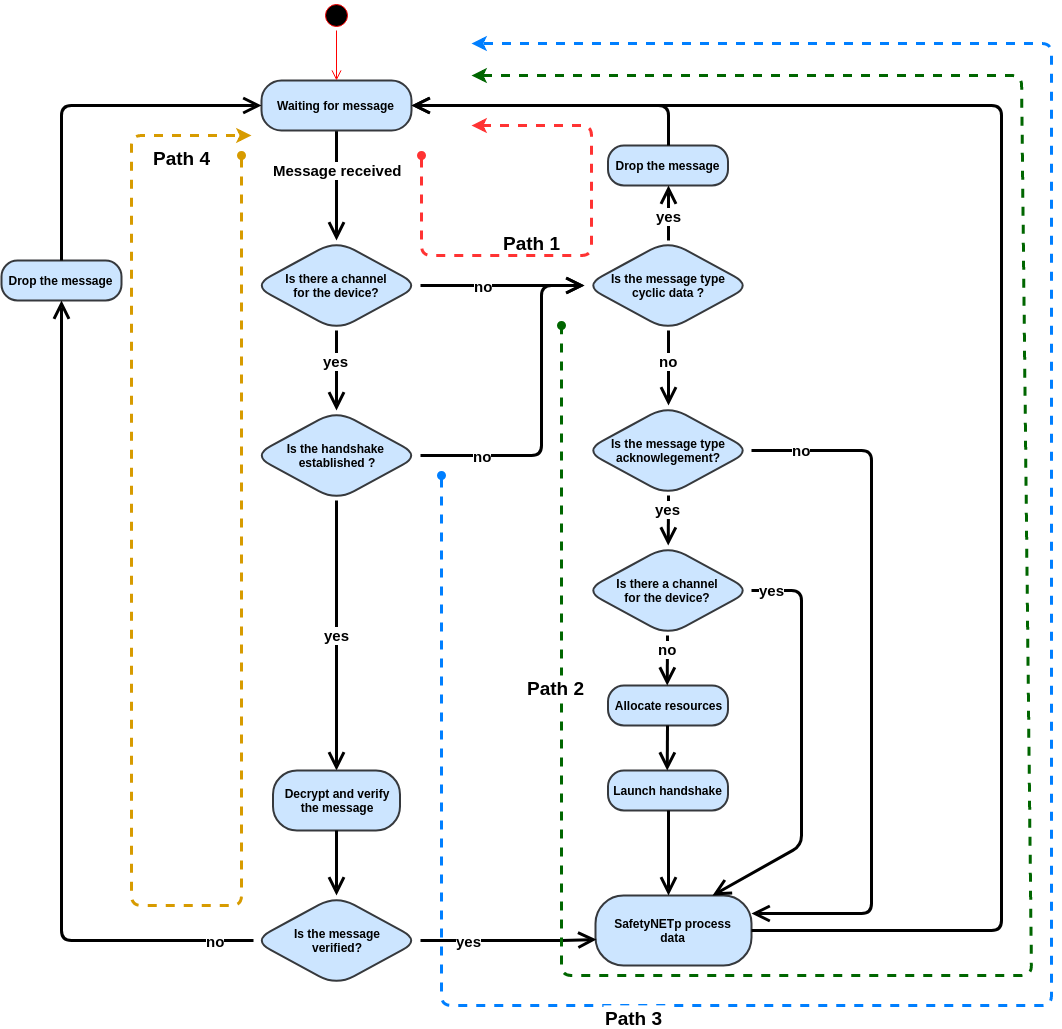
\includegraphics[height=16cm]{figures/design/incoming_messages_flowtchart.jpg}
\caption{Flowchart for incoming messages}\label{incoming_messages_flowtchart}
\end{figure}
\newpage

\subsection{First Subscription Vulnerability}

Triggered by the first handshake process, the devices establish the DTLS handshake and start exchanging
data securely. The trigger for establishing the handshake could not be secured as no secure channel exists
before establishing the handshake. Therefore we are obliged to perform the first subscription unprotected as it is the trigger.
We already mentioned the issues of sending unprotected subscribe requests. Fake \textit{subscribe requests} could be sent
which results on exchanging unnecessary data in the network. We already proposed a solution for securing subscribe requests
after the secure channel is provided, however, we did not discuss the first subscription issue.

When the system starts up, before any message is exchanged, an attacker could easily impersonate the identity
of a device and send a \textit{subscribe request} with its identity. The device which has the topic will send back a
subscribe acknowledgment as response and both devices will establish the handshake. As the first subscription is
forged by the attacker, the \textit{cyclic data} sent by the publisher is not needed by the subscriber.

In order to avoid receiving the unnecessary cyclic data, we propose two solutions.
After that the handshake is established, we reset the application state of the two parts the publisher and the subscriber.
By resetting the application state, both the publisher and the subscriber forget about the previous subscriptions
and they perform the subscription process another time. Therefore, if the first subscription is fake, by resetting the
application state, no \textit{cyclic data} for the fake subscription will be sent and all the new subscription could be performed
securely using the available channel. In fact, this solution could not be applied currently, as SafetyNETp does not provide
an API for resetting the application. However, The solution is interesting and we could ask SafetyNETp developers for such API to solve the problem.

The second solution consists of changing the handshake timing previously discussed and perform the handshake
at the second position shown in \autoref{when_to_establish_the_handshake}. In this case, when a \textit{subscribe request} is
received, our security layer don't pass the message to SafetyNETp to be processed. Because if the topic exists
the device will send a \textit{subscribe acknowledgment} and start sending \textit{cyclic data} which could be unnecessary as
the subscription is not protected. Not passing the \textit{subscribe request} to SafeyNETp allows avoiding this issue.
The device which sends a \textit{subscribe request} activates a server and the receiving device after verifying that the topic exists,
takes the client role and start establishing the handshake with the subscriber. Using this method no subscribe acknowledgment
is sent before establishing the handshake, therefore, no \textit{cyclic data} is sent. After finishing the handshake, our security
layer let SafetyNETp process \textit{subscribe requests} and all the message could be exchanged securely. The problem with this
method is that our security layer is not able to know whether a topic exists or not without letting SafetyNETp process
subscribe requests. In fact, for our security layer, the indicator for the topic existence is the subscribe acknowledgment.
It is not possible to detect whether a topic exists or not without seeing a subscribe acknowledgment. Therefore to make
this possible, SafetyNETp developers need to provide a function which returns whether a topic exists having a subscribe
request as input.

To conclude, the first subscription process is currently performed without protection and the problem
could be solved using one of the cited solutions if SafetyNETp developers could provide the needed APIs.


\subsection{Keying Materials Renewal}

Cryptology is a mathematical science which contains two branches, cryptography, and cryptanalysis.
The main goal of cryptography is to ensure data confidentiality by encrypting an input message called
plaintext to obtain an encrypted output called ciphertext. The obtained ciphertext is unreadable and it can
be decrypted only by parts that have the secret key used for encryption. However, the cryptanalysis
goal is to gain as much information as possible about the original unencrypted data. Cryptanalysis
can lead to decrypt ciphertexts without having the secret key and much worse it can even lead to figure it out. This achieved by several technics, for example, analyzing a huge number of ciphertexts.
This technic is called cryptanalysis with ciphertext-only, which mean that the attacker knows only ciphertexts \cite{Cryptology}.

Our security layer provides authentication, confidentiality, and integrity. These three services rely on keeping the keying
material being used secret. In SafetyNETp networks, using our security layer, publishers send each cycle
encrypted \textit{cyclic data} messages to its subscribers. An untrusted third party can easily obtain a huge number of
encrypted messages which allows him to perform cryptanalysis studies in order to break the encryption.
If the keying materials are compromised, encrypted messages can be decrypted by an attacker, the messages
can be modified without detecting the modification, an attacker will be able to impersonate
the identity of a device legitimately.

The cryptanalysis relies on studying the encrypted traffic which needs a huge amount of encrypted message
and another important factor which is time. To avoid this kind of attacks, we can simply renew
the keying materials by running a new handshake every period of time.
This period should be defined based on how much time an attacker needs to be able to break the encryption.
Once the period is defined, each two communicating devices run a new handshake upon the expiry of the period.
\autoref{keying_materials_renewal} illustrates how keying material renewal is performed. After that the first handshake has been
established, a timeout is set and \textit{cyclic data} is sent using the first provided keying material or in other words the first DTLS context.
Upon the timeout expiry, a new handshake is established in parallel while sending \textit{cyclic data}.
When the new handshake is established, we can choose whether to switch directly to use the new DTLS context
or to wait for a period of time before switching like shown the figure. At each handshake, the timer is reset
and upon its expiry, a new handshake is established and therefore we can minimize the possibility of cryptanalysis attacks.

\begin{figure}[H]
\centering
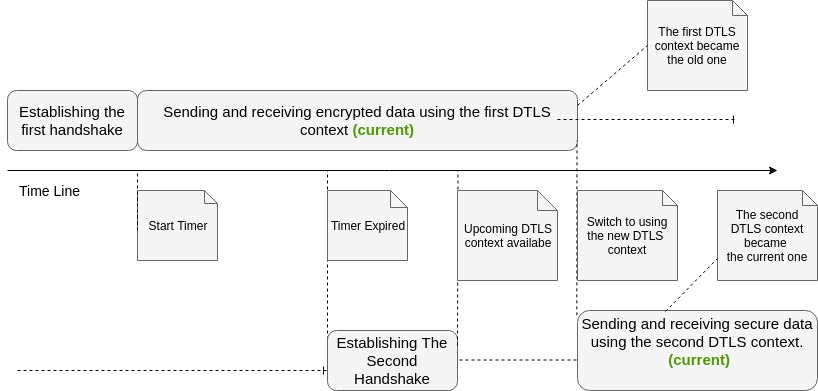
\includegraphics[height=7cm]{figures/design/keying_materials_renewal.jpg}
\caption{Keying Materials Renewal}\label{keying_materials_renewal}
\end{figure}

\subsection{Session Closing}

When no more data need to be exchanged between two devices, the session should be closed and the allocated resources
for the handshake establishment and keying materials should be freed. A session could be closed for several reasons.

First, the subscriber could unsubscribe from all the topics received from a certain publisher, therefore, there will be no more
data published to the subscriber. Hence the secure channel is not needed anymore. At this level, the session can be closed and
the resources can be liberated. In each device, we need to keep track of the topics being used and once no topic is being communicated
the session should be closed. In each Publisher/Subscriber relation, the topics are counted as follows. The subscriber increments
the number of topics being used each time it receives a \textit{subscribe acknowledgment} from the publisher. The subscriber decrements the number
if it receives an \textit{unpublished} message from the publisher or after having sent an \textit{unsubscribe request}. The publisher applies
the same principle, it increments the number after sending a \textit{subscribe acknowledgment} and decrements the number if it receives
an \textit{unsubscribe request} or after sending an \textit{unpublished} message. In every device when the number of topics being used for a session is equal to
zero, the session will be closed. This works fine if we assume that messages are sent reliably, however, if we consider using unreliable
transport we will have issues. Assuming we have a subscriber and a publisher and the subscriber is subscribed for just one single topic,
the number of topics being used on both sides is equal to one. If the subscriber sends an \textit{unsubscribe request} to the publisher and the message is lost,
the subscriber decrements the number of topics being used to become zero which is not the case for the publisher (the message is lost).
In this case, we end up having different numbers on each side and only the subscriber closes the session. Alongside counting the topics,
we add another condition to avoid this desynchronization. A session should be closed if two conditions are satisfied.
For the subscriber, the number of topics being used should be equal to zero and in addition, no \textit{cyclic data} is received. In fact, if the
subscriber still receives \textit{cyclic data} means that there has been a packet loss. Hence the subscriber can resend the \textit{unsubscribe request} until the publisher
stops sending \textit{cyclic data}. For the publisher case, the session should be closed, like the subscriber, if the number of topics
being used is equal to zero and if no \textit{still alive} messages are being received.
% In fact, if the publisher sends an \textit{unpublished}
% message for the last topic and the subscriber is still sending \textit{still alive} messages means that the \textit{unpublished} message is lost and hence it could retransmit the message.

The second case for which a session should be closed is that one of both sides is not working anymore (the devices crashes
or reboots for example). After finishing subscription process, \textit{still alive} messages are sent periodically by the subscriber
to the publisher, hence, if the publisher does not receive \textit{still alive} messages for a well-defined timeout (defined by SafetyNETp application layer),
it considers that the subscriber is down. When the \textit{still alive} message timeout expires, the session should be closed.
Regarding the subscriber, it considers that the publisher is down if it does not receive \textit{cyclic data} messages for also a well-defined timeout (defined by SafetyNETp application layer).
When the timeout expires, the subscriber should close the session.

The last case is when performing a handshake. Whether it is the first handshake or a handshake for session renewal,
if the handshake fails, the session should be closed.

We can have the situation where a publisher and a subscriber have just closed their session
and the subscriber decides to get subscribed another time. As the session was closed, they
need to re-establish the handshake in order to communicate. To avoid this situation, if no
communication is needed between the publisher and the subscriber, the session will not be closed
immediately. Instead, a timeout will be set and the session will be closed when the timeout expires.
This allows more flexibility. While the timeout is not expired,
the session will still open and could be used for a new communication. Hence, no need for a new handshake.

\subsection{Frame Layout}

After that the handshake is established SafetyNETp messages are no more sent as plaintext, instead, they
are sent encrypted and encapsulated into DTLS frames. In order to minimize the possibility of cryptanalysis attacks,
we decided to run a new handshake each a well defined period to renew the keying materials being used.
Due to reordering, it is still possible to receive DTLS frames encrypted by the old keying material
from the previous handshake. Therefore, we are not able to know whether a DTLS frame is encrypted
using the new or the old keying material. Hence the receiving device will not be able to decrypt
and verify messages.

In order to solve this issue, our solution is to add additional information to the message to indicate which keying material was
used for encryption. In fact, this consists of adding a one-byte field before the DTLS frame. This field is incremented each
time the handshake is established. We call this field channel id and according to its value, the receiving device could decide
which keying material to use to decrypt and verify the message.


% The first solution consists of using the DTLS epoch. In fact, the epoch is a one-byte integer field in DTLS frame header.
% After each established handshake, DTLS increments the epoch field to indicate that the keying material
% being used had been renewed. Therefore, the receiving devices will be able to know which keying material
% was used based on the epoch field. In DTLS version 1.2, the epoch value starts from zero and at
% each new handshake, it is incremented. Unfortunately, relying on a DTLS header field means that
% our security will be dependent on the DTLS header format. This dependency can cause a problem in the future
% if new versions of DTLS modifies the header format or how a field is being used. That's why we should use DTLS
% as a black box to avoid any dependency. Hence, if the DTLS header changes, nothing will affect our security
% layer and the design will remain the same. Furthermore, the epoch field is already used differently in DTLS version 1.3 \cite{draftTLSv1.3}
% which still being developed. In version 1.3 the epoch field starts from four instead of zero.

% The second solution is to add additional information in the message to indicate which keying material was
% used for encryption. In fact, this consists of adding a one-byte field before the DTLS frame. This field is incremented each time the handshake is established. We call
% this channel id and according to its value, the receiving device could decide which keying material to use
% to decrypt and verify the message.

% Comparing the two solutions, the second lead to more bandwidth usage by adding additional information into
% the message whereas the first does not include any additional information. However, using the first
% solution creates a dependency between our security layer's design and DTLS's design whereas the second
% solution does not. Hence, the security layer will not be affected by changing the DTLS design in this case.
% Therefore we use the second solution.

\autoref{security_layer_frame_layoutl} shows the security layer frame layout. The first byte indicates that the message is a secured
frame, the second byte is channel id which indicates which keying material was used for encryption. The rest
of the message is the encrypted DTLS frame which encapsulates SafetyNETp application layer message.

\begin{figure}[H]
\centering
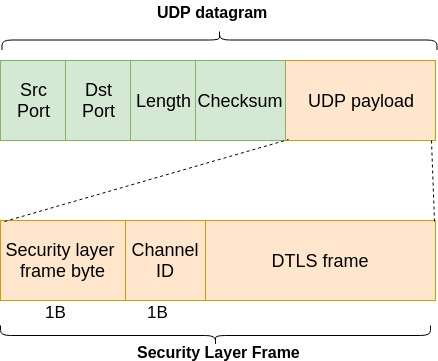
\includegraphics[height=6.5cm]{figures/design/Security_layer_frame_layout.jpg}
\caption{The security layer frame layout}\label{security_layer_frame_layoutl}
\end{figure}

\section*{Conclusion}

Throughout this chapter, we presented the global and the detailed design where we introduced
the existing problems, we provided the candidate alternatives and chose the solutions we judge suitable
for our case.
